%%%%%%%%%%%%%%%%%%%%%%%%%%%%%%%%%%%%%%%%%%  不使用 authblk 包制作标题  %%%%%%%%%%%%%%%%%%%%%%%%%%%%%%%%%%%%%%%%%%%%%%
%-------------------------------PPT Title-------------------------------------
\title{08-\rm{VASP}中的\rm{PAW}方法}
%-----------------------------------------------------------------------------
%----------------------------Author & Date------------------------------------

%\author[\textrm{Jun\_Jiang}]{姜\;\;骏\inst{}} %[]{} (optional, use only with lots of authors)
%% - Give the names in the same order as the appear in the paper.
%% - Use the \inst{?} command only if the authors have different
%%   affiliation.
%\institute[BCC]{\inst{}%
\institute[Gain~Strong]{\inst{}%
%\vskip -20pt 北京市计算中心}
\vskip -20pt {\large 格致斯创~科技}}
\date[\today] % (optional, should be abbreviation of conference name)
{%	{\fontsize{6.2pt}{4.2pt}\selectfont{\textcolor{blue}{E-mail:~}\url{jiangjun@bcc.ac.cn}}}
\vskip 45 pt {\fontsize{8.2pt}{6.2pt}\selectfont{%清华大学\;\;物理系% 报告地点
	\vskip 5 pt \textrm{2023.03.11}}}
}

%% - Either use conference name or its abbreviation
%% - Not really information to the audience, more for people (including
%%   yourself) who are reading the slides onlin%%   yourself) who are reading the slides onlin%%   yourself) who are reading the slides onlineee
%%%%%%%%%%%%%%%%%%%%%%%%%%%%%%%%%%%%%%%%%%%%%%%%%%%%%%%%%%%%%%%%%%%%%%%%%%%%%%%%%%%%%%%%%%%%%%%%%%%%%%%%%%%%%%%%%%%%%

\subject{}
% This is only inserted into the PDF information catalog. Can be left
% out.
%\maketitle
\frame
{
%	\frametitle{\fontsize{9.5pt}{5.2pt}\selectfont{\textcolor{orange}{“高通量并发式材料计算算法与软件”年度检查}}}
\titlepage
}
%-----------------------------------------------------------------------------

%------------------------------------------------------------------------------列出全文 outline ---------------------------------------------------------------------------------
%\section*{}
%\frame[allowframebreaks]
%{
%  \frametitle{Outline}
%%  \frametitle{\textcolor{mycolor}{\secname}}
%  \tableofcontents%[current,currentsection,currentsubsection]
%}
%%在每个section之前列出全部Outline
%%类似的在每个subsection之前列出全部Outline是\AtBeginSubsection[]
%\AtBeginSection[]
%{
%  \frame<handout:0>%[allowframebreaks]
%  {
%    \frametitle{Outline}
%%全部Outline中,本部分加亮
%    \tableofcontents[current,currentsection]
%  }
%}

%-----------------------------------------------PPT main Body------------------------------------------------------------------------------------
\small
%\section{\rm{VASP~}软件中\rm{PAW~}计算的实现}
%\frame
%
%	\frametitle{\textrm{VASP}计算的特色}
%	相比于与普通的第一原理计算软件,\textrm{VASP}很好地平衡了计算效率和精度的问题,总的来说,\textrm{VASP}主要通过这几个特色保证了计算的高效能
%	\begin{itemize}
%	     \item 迭代与优化算法的多样性\\
%		     本质上电荷密度迭代 \textrm{\&\&} 体系总能量优化是相同的优化问题,采用了类似的算法\upcite{CMS6-15_1996,PRB54-11169_1996}:\\
%			\textcolor{blue}{\textrm{Pseudo-Newton、Conjugate-Gradient、Broyden~mix、damping-factor、RMM-DIIS}}
%	     \item 尽可能采用局域基(原子轨道基)函数:~\\
%		     \textcolor{blue}{\textrm{LREAL}}=\textcolor{red}{\textrm{.TRUE.}}\\
%			优化的投影函数也尽可能在实空间表示
%	     \item \textrm{PAW}原子数据集:\textcolor{blue}{优异的赝势}\upcite{PRB59-1758_1999}
%	\end{itemize}
%}

\frame
{
%	\frametitle{\textrm{PAW}原子数据集}
	\frametitle{\textrm{PAW Augmentation}}
\begin{figure}[h!]
\centering
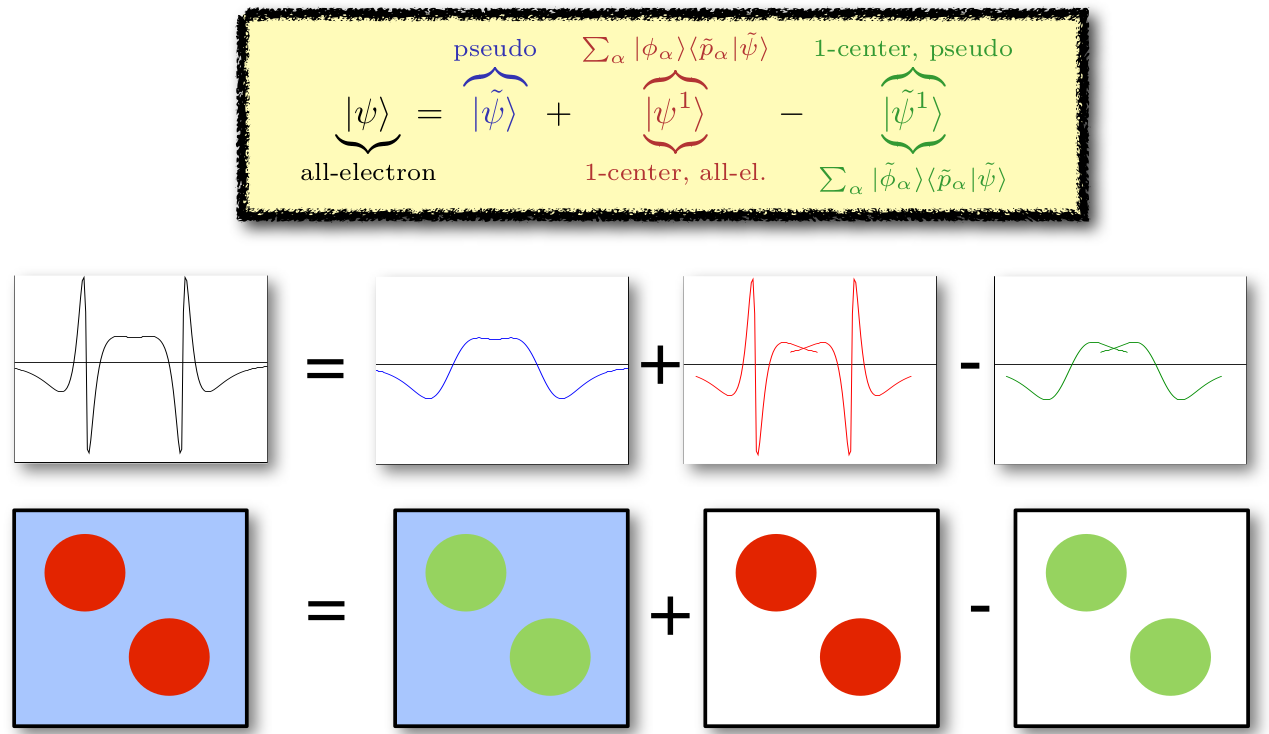
\includegraphics[height=2.3in,width=4.0in,viewport=0 0 1280 745,clip]{Figures/PAW-baseset.png}
\caption{\tiny \textrm{The Augmentation of PAW.}}%(与文献\cite{EPJB33-47_2003}图1对比)
\label{PAW_baseset}
\end{figure}
}

%\frame
%{
%	\frametitle{\textrm{PAW Augmentation}}
%\begin{figure}[h!]
%\centering
%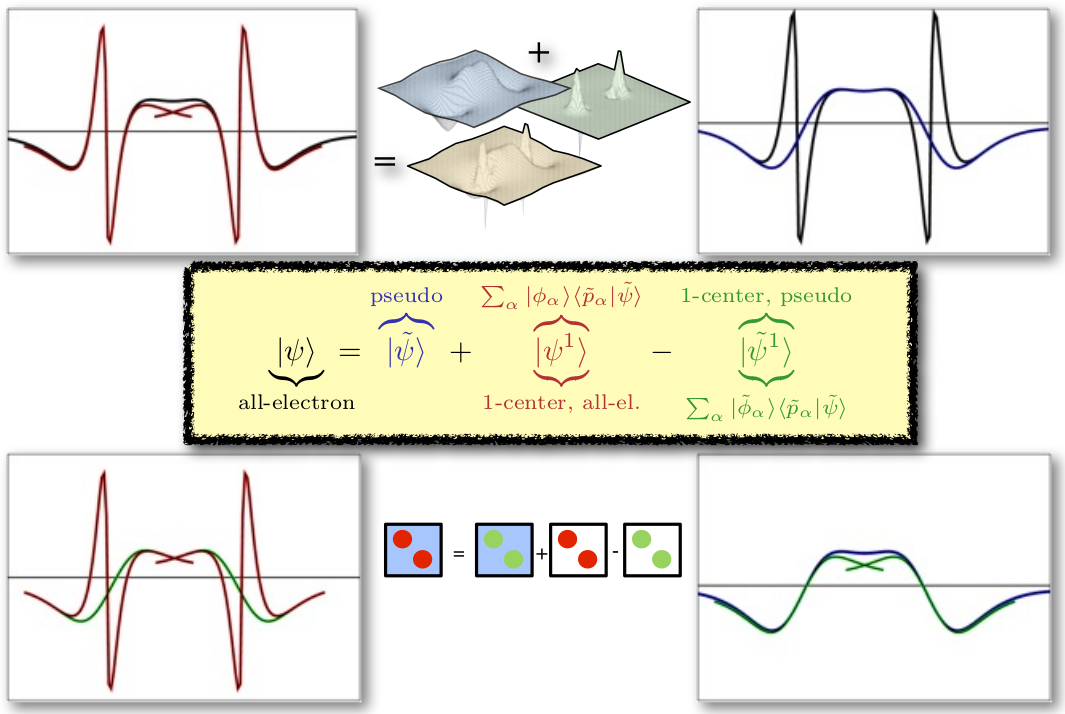
\includegraphics[height=2.3in,width=4.0in,viewport=0 0 1100 745,clip]{Figures/PAW-projector.png}
%\caption{\tiny \textrm{The projector of PAW.}}%(与文献\cite{EPJB33-47_2003}图1对比)
%\label{PAW_projector}
%\end{figure}
%}

\frame
{
\frametitle{电荷密度的重新分解}
\textrm{PAW}方法提出后有很长一段时间没有能够得到广泛应用,直到\textrm{G. Kresse}等将\textrm{Bl\"ochl}的原始方案中电荷密度计算方案重新组合后,明确了\textrm{PAW}方法与\textrm{USPP}方法的内在联系。
\begin{itemize}
	\item 芯层电荷与核电荷构成离子实电荷:$n_{Zc}=n_Z+n_c$
\end{itemize}
\begin{figure}[h!]
\centering
\vspace{-10.5pt}
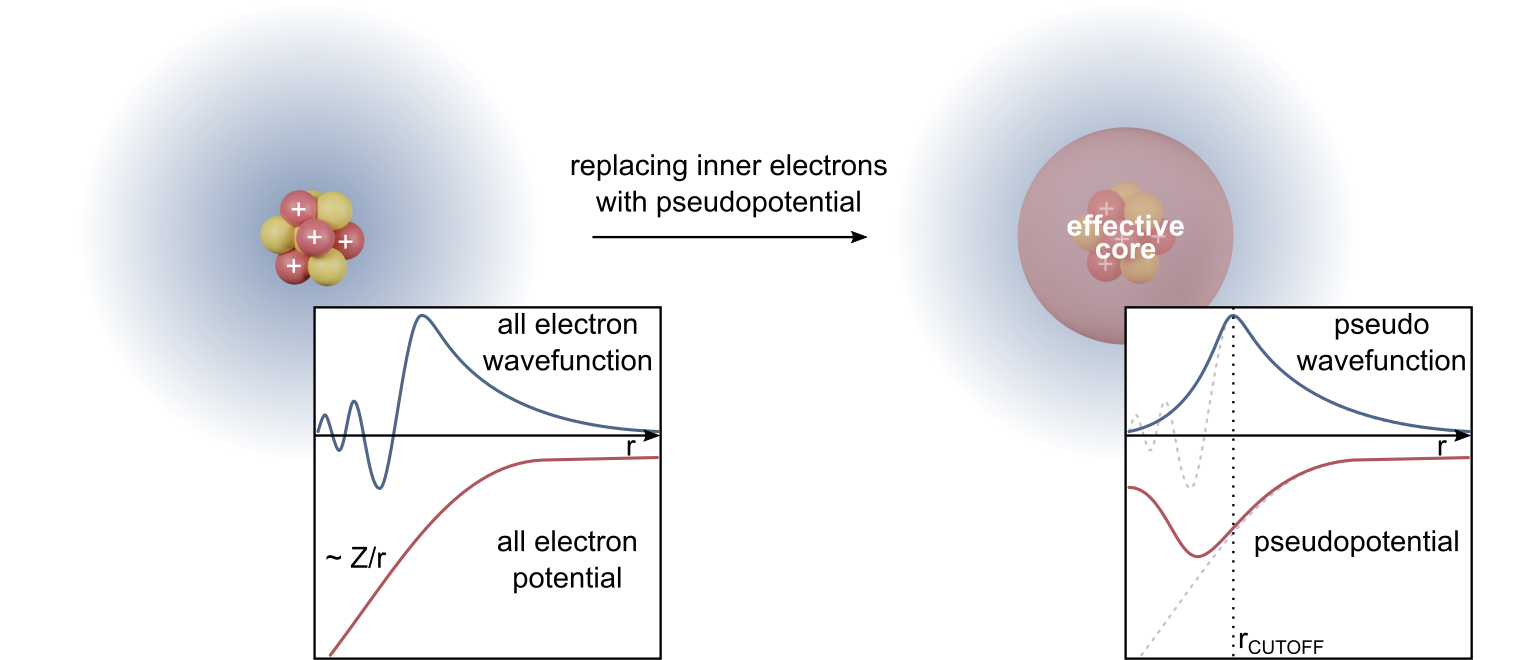
\includegraphics[height=1.5in,width=3.0in,viewport=0 0 380 190,clip]{Figures/Pseudo-potential_charge.png}
\caption{\tiny \textrm{The difference of the electron-density distributing from P.~Bl\"ochl  and from G.~Kresse.}}%(与文献\cite{EPJB33-47_2003}图1对比)
\label{PAW_Pseudo-Charge}
\end{figure}
}

\frame
{
	\frametitle{电荷密度重新分解与赝势}
\begin{itemize}
	\item 赝离子实电荷要满足的条件$$\int_{\Omega_c}n_{Zc}(\vec r)\mathrm{d}^3\vec r=\int_{\Omega_c}\tilde n_{Zc}(\vec r)\mathrm{d}^3\vec r$$
\end{itemize}
在此基础上,\textrm{Bl\"ochl}方案中的电荷可以重新分解为:
\begin{displaymath}
	\begin{aligned}
		n_T=n+n_{Zc}\equiv&\underbrace{(\tilde n+\hat n+\tilde n_{Zc})}\\
		&\quad\qquad\textcolor{blue}{\tilde n_T}\\
				  &+\underbrace{(n^1+\hat n+n_{Zc})}-\underbrace{(\tilde n^1+\hat n+\tilde n_{Zc})}\\
				  &\quad\qquad \textcolor{blue}{n_T^1}\qquad\qquad\qquad\textcolor{blue}{\tilde n_T^1}
	\end{aligned}
\end{displaymath}
\textcolor{red}{注意}:~\textrm{G. Kresse}方案中补偿电荷$\hat n$局域在每个缀加球内。
}

\frame
{
	\frametitle{\textrm{Hartree~}势的分解}
\begin{displaymath}
	\begin{aligned}
		\dfrac12(n_T)(n_T)=&\dfrac12(\tilde n_T)(\tilde n_T)+(n_T^1-\tilde n_T^1)(\tilde n_T)\\
				&+\dfrac12(n_T^1-\tilde n_T^1)(n_T^1-\tilde n_T)
	\end{aligned}
\end{displaymath}
这里$$(a)(b)=\int\mathrm{d}\vec r\mathrm{d}\vec r^{\prime}\dfrac{a(\vec r)b(\vec r\,^{\prime})}{|\vec r-\vec r\,^{\prime}|}$$
\textcolor{red}{近似}:$\tilde n_T$用$\tilde n_T^1$替换:
\begin{displaymath}
	\dfrac12(n_T)(n_T)=\textcolor{blue}{\dfrac12(\tilde n_T)(\tilde n_T)}\textcolor{magenta}{-\dfrac12\overline{(\tilde n_T^1)(\tilde n_T^1)}}+\textcolor{purple}{\dfrac12\overline{(n_T^1)(n_T^1)}}
\end{displaymath}
这里$$\overline{(a)(b)}=\int_0^{\mathrm{r}_c}\mathrm{d}\vec r\mathrm{d}\vec r^{\prime}\dfrac{a(\vec r)b(\vec r\,^{\prime})}{|\vec r-\vec r\,^{\prime}|}$$
}

\frame
{
	\frametitle{}
	{\fontsize{7.2pt}{5.2pt}\selectfont{具体地,将$\tilde n_T$代入表达式并展开,有
	\begin{enumerate}
	\item 第一项	
	\begin{displaymath}
		\begin{aligned}
			&\textcolor{blue}{\dfrac12(\tilde n+\hat n)(\tilde n+\hat n)+(\tilde n_{Zc})(\tilde n+\hat n)+\dfrac12(\tilde n_{Zc})(\tilde n_{Zc})}\\
			=&\dfrac12(\tilde n+\hat n)(\tilde n+\hat n)+(\tilde n_{Zc})(\tilde n+\hat n)\boxed{\textcolor{red}{+\dfrac12\overline{(\tilde n_{Zc})(\tilde n_{Zc})}}}\\
			&+U(\mathbf{R},Z_{\mathrm{ion}})
		\end{aligned}
	\end{displaymath}
这里假设不同原子彼此间芯电荷不发生重叠
	\item 第二项
	\begin{displaymath}
		\textcolor{magenta}{-\dfrac12\overline{(\tilde n^1+\hat n)(\tilde n^1+\hat n)}-\overline{(\tilde n_{Zc})(\tilde n^1+\hat n)}}\boxed{\textcolor{red}{-\dfrac12\overline{(\tilde n_{Zc})(\tilde n_{Zc})}}}
	\end{displaymath}
	\item 第三项
\begin{displaymath}
	\textcolor{purple}{\dfrac12\overline{(\tilde n^1)(\tilde n^1)}+\overline{(\tilde n_{Zc})(\tilde n^1)}}\boxed{\textcolor{red}{+\dfrac12\overline{(\tilde n_{Zc})(\tilde n_{Zc})}}}
\end{displaymath}
	\end{enumerate}
	注意到第一项展开中$U(\mathbf{R},Z_{\mathrm{ion}})$表示的是均匀静电场背景下点电荷$Z_{\mathrm{ion}}$的静电相互作用,$\dfrac12\overline{(\tilde n_{Zc})(\tilde n_{Zc})}$表示离子实的自相互作用,这部分将与第二项展开式中对应部分彼此抵消,而第三项中$\dfrac12\overline{(\tilde n_{Zc})(\tilde n_{Zc})}$并未包括在最后的总能量表达式中,因为这部分能量只是影响了能量零点位置的选择%,最后用\textrm{Ewald}求和计算
}}}

\frame
{
\frametitle{交换-相关能泛函的处理}
\textrm{G. Kresse}方案中电荷密度分解为
\begin{displaymath}
	n_c+n=(\tilde n+\hat n+\tilde n_c)+(n^1+n_c)-(\tilde n^1+\hat n+\tilde n_c)
\end{displaymath}
对比原始的\textrm{Bl\"ochl}方案中电荷分解为
\begin{displaymath}
	n_c+n=(\tilde n)+(n^1+n_c)-(\tilde n^1)
\end{displaymath}
%\textrm{G. Kresse}方案中赝离子实电荷$\tilde n_{Zc}$与\textrm{Bl\"ochl}方案中$\tilde n_c$的约束条件不同,

显然,\textrm{VASP}中的交换-相关能计算表达式
\begin{displaymath}
	E_{\mathrm{XC}}[\tilde n+\hat n+\tilde n_c]+\overline{E_{\mathrm{XC}}[n^1+n_c]}-\overline{E_{\mathrm{XC}}[\tilde n^1+\hat n+\tilde n_c]}
\end{displaymath}
但由于交换-相关能泛函是非线性的,\textrm{G. Kress}的电荷分解引起的误差则为
\begin{displaymath}
	\begin{aligned}
		&\textcolor{blue}{\overline{E_{\mathrm{XC}}[(\tilde n+\hat n+\tilde n_c)+(n^1+n_c)-(\tilde n^1+\hat n+\tilde n_c)]}}\\
		&-\overline{E_{\mathrm{XC}}[\tilde n+\hat n+\tilde n_c]}-\overline{E_{\mathrm{XC}}[n^1+n_c]}+\overline{E_{\mathrm{XC}}[\tilde n^1+\hat n+\tilde n_c]}
	\end{aligned}
\end{displaymath}
}

\frame
{
	\frametitle{总能量表达式}
	最终完成体系总能量的表达式,根据总能量表达式$$E=\tilde E+E^1-\tilde E^1$$其中
	\begin{displaymath}
		\begin{aligned}
			\tilde E=&\sum_nf_n\langle\tilde\Psi_n|-\frac12\nabla^2|\tilde\Psi_n\rangle+E_{\mathrm{XC}}[\tilde n+\hat n+\tilde n_c]+E_H[\tilde n+\hat n]\\
			&+\int \textcolor{magenta}{v_H[\tilde n_{Zc}]}[\tilde n(\vec r)+\hat n(\vec r)]\mathrm{d}\vec r+U(\vec R,Z_{\mathrm{ion}})\\
			\tilde E^1=&\sum_{(i,j)}\rho_{ij}\langle\tilde\phi_i|-\frac12\nabla^2|\tilde\phi_j\rangle+\textcolor{purple}{\overline{E_{\mathrm{XC}}[\tilde n^1+\hat n+\tilde n_c]}+\overline{E_H[\tilde n^1+\hat n]}}\\
			&+\int_{\Omega_r}\textcolor{magenta}{v_H[\tilde n_{Zc}]}[\tilde n^1(\vec r)+\hat n(\vec r)]\mathrm{d}\vec r
		\end{aligned}
	\end{displaymath}
}

\frame
{
	\frametitle{总能量表达式}
	\begin{displaymath}
		\begin{aligned}
			E^1=&\sum_{(i,j)}\rho_{ij}\langle\phi_i|-\frac12\nabla^2|\phi_j\rangle+\overline{E_{\mathrm{XC}}[n^1+n_c]}+\overline{E_H[n^1]}\\
			&+\int_{\Omega_r}v_H[n_{Zc}]n^1(\vec r)\mathrm{d}\vec r
		\end{aligned}
	\end{displaymath}
	$v_H$是电荷密度$n$产生的静电势
	$$v_H[n](\vec r)=\int\dfrac{n(\vec r\,^{\prime})}{|\vec r-\vec r\,^{\prime}|}\mathrm{d}\vec r\,^{\prime}$$
	$E_H[n]$是对应的静电能
	$$E_H[n]=\dfrac12(n)(n)=\dfrac12\int\mathrm{d}\vec r\mathrm{d}\vec r\,^{\prime}\dfrac{n(\vec r)n(\vec r\,^{\prime})}{|\vec r-\vec r\,^{\prime}|}$$ 
	$U(\vec R,Z_{\mathrm{ion}})$\textcolor{blue}{由\textrm{Ewald}求和计算}
}

\frame
{
	\frametitle{补充电荷的构造}
	根据约束条件
	\begin{displaymath}
		\int_{\Omega_c}(n^1-\tilde n^1-\hat n)|\vec r-\vec R|^lY_{lm}^{\ast}(\widehat{\vec r-\vec R})\mathrm{d}\vec r=0
	\end{displaymath}
	定义电荷密度差
	\begin{displaymath}
		Q_{ij}(\vec r)=\phi_i^{\ast}(\vec r)\phi_j(\vec r)-\tilde\phi_i^{\ast}(\vec r)\tilde\phi_j(\vec r)
	\end{displaymath}
	电荷密度差的多极矩为
	\begin{displaymath}
		q_{ij}^L(\vec r)=\int_{\Omega_r}Q_{ij}(\vec r)|\vec r-\vec R|^lY_{lm}^{\ast}(\widehat{\vec r-\vec R})\mathrm{d}\vec r
	\end{displaymath}
	因此,补充电荷的计算为:
	\begin{displaymath}
		\begin{aligned}
			\hat n=\sum_{(i,j),L}\sum_n f_n\langle\tilde\Psi_n|\tilde p_i\rangle\langle\tilde p_j|\Psi_n\rangle\hat Q_{ij}^L(\vec r)\\
			\hat Q_{ij}^L(\vec r)=q_{ij}^Lg_l(|\vec r-\vec R|)Y_{lm}(\widehat{\vec r-\vec R})
		\end{aligned}
	\end{displaymath}
}

\frame
{
	\frametitle{重叠矩阵和\textrm{Hamiltonian~}的构造}
重叠矩阵
	\begin{displaymath}
		\langle\tilde\Psi_n|\mathbf{S}|\tilde\Psi_m\rangle=\delta_{nm}
	\end{displaymath}
	其中重叠矩阵$$S[\{\mathbf{R}\}]=1+\sum_i|\tilde p_i\rangle q_{ij}\langle\tilde p_j|$$
	而$$q_{ij}=\langle\phi_i|\phi_j\rangle-\langle\tilde\phi_i|\tilde\phi_j\rangle$$
	\textrm{Hamiltonian}的计算
	\begin{displaymath}
		H[\rho,\{\mathbf{R}\}]=-\dfrac12\nabla^2+\tilde v_{e\!f\!f}+\sum_{(i,j)}|\tilde p_i\rangle(\hat D_{ij}+D_{ij}^1-\tilde D_{ij}^1)\langle\tilde p_j|	
	\end{displaymath}
	$$\tilde v_{e\!f\!f}=v_H[\tilde n+\hat n+\tilde n_{Zc}]+v_{\mathrm{XC}}[\tilde n+\hat n+\tilde n_{Zc}]$$
}

\frame
{
	\frametitle{重叠矩阵和\textrm{Hamiltonian~}的构造}
	$$\hat D_{ij}=\dfrac{\partial\tilde E}{\partial\rho_{ij}}=\int\dfrac{\delta\tilde E}{\delta\hat n(\vec  r)}\dfrac{\partial\hat n(\vec r)}{\partial\rho_{ij}}\mathrm{d}\vec r=\sum_{L}\int\tilde v_{e\!f\!f}\hat Q_{ij}^L(\vec r)\mathrm{d}\vec r$$
	$$D_{ij}^1=\dfrac{\partial E^1}{\partial\rho_{ij}}=\langle\phi_i|-\dfrac12\nabla^2+v_{e\!f\!f}^1|\phi_j\rangle$$
	其中$$v_{e\!f\!f}^1[n^1]=v_H[n^1+n_{Zc}]+v_{\mathrm{XC}}[n^1+n_c]$$
	$$\tilde D_{ij}^1=\dfrac{\partial\tilde E^1}{\partial\rho_{ij}}=\langle\tilde\phi_i|-\dfrac12\nabla^2+\tilde v_{e\!f\!f}^1|\tilde\phi_j\rangle+\sum_L\int_{\Omega_r}\mathrm{d}\vec r\tilde v_{e\!f\!f}^1(\vec r)\hat Q_{ij}^L$$
	其中$$\tilde v_{e\!f\!f}^1[\tilde n^1]=v_H[\tilde n^1+\hat n+\tilde n_{Zc}]+v_{\mathrm{XC}}[\tilde n^1+\hat n+\tilde n_c]$$
}

\frame
{
	\frametitle{\textrm{Double counting correlations}}
	能带计算中,总能量可通过\textrm{Kohn-Sham}本征值求和扣除\textrm{Double counting}计算更方便,其中修正项
	\begin{displaymath}
		\begin{aligned}
			\tilde E_{dc}=&-E_H[\tilde n+\hat n]+E_{\mathrm{XC}}[\tilde n+\hat n+\tilde n_c]\\
			&-\int v_{\mathrm{XC}}[\tilde n+\hat n+\tilde n_c](\tilde n+\hat n)\mathrm{d}\vec r\\
			E_{dc}^1=-\overline{E_H[n^1]}&+\overline{E_{\mathrm{XC}}[n^1+n_c]}-\int_{\Omega_r}v_{\mathrm{XC}}[n^1+n_c]n^1\mathrm{d}\vec r\\
			\tilde E_{dc}^1=&-\overline{E_H[\tilde n^1+\hat n]}+\overline{E_{\mathrm{XC}}[\tilde n^1+\hat n+\tilde n_c]}\\
			&-\int v_{\mathrm{XC}}[\tilde n^1+\hat n+\tilde n_c](\tilde n^1+\hat n)\mathrm{d}\vec r
		\end{aligned}
	\end{displaymath}
	因此总能量的计算表达式是
	$$E=\sum_nf_n\langle\tilde\Psi_n|H|\tilde\Psi_n\rangle+\tilde E_{dc}+E_{dc}^1-\tilde E_{dc}^1+U(\vec R,Z_{\mathrm{ion}})$$
}

\subsection{\rm{PAW}方法与\rm{US-PP}的关系}
\frame
{
	\frametitle{\textrm{PAW}与\textrm{US-PP}近似}
	\textrm{G. Kresse}指出只要总能量表达式中$E^1$和$\tilde E^1$在原子构象附近作线性化即可得到\textrm{US-PP}的表达式。
	
	如果电子占据数$\rho_{ij}$直接用原子态构象$\rho_{ij}^a$近似,因此电荷密度分布记作$n_a^1$、$\tilde n_a^1$和$\hat n_a$,则$E^1$中的\textcolor{blue}{\underline{\textrm{Hartree}能和交换-相关能项}}在$n_a$附近线性化($n_a\Rightarrow n_a^1$):
	\begin{displaymath}
		E_{\mathrm{XC}}(\textcolor{red}{n_a^1+n_c})+E_H(\textcolor{red}{n_a^1})+\int(v_{\mathrm{XC}}[\textcolor{red}{n_a^1+n_c}]+v_H[\textcolor{red}{n_a^1}])[n^1(\vec r)-\textcolor{red}{n_a^1(\vec r)}]\mathrm{d}\vec r
	\end{displaymath}
	在\textrm{PAW}方法中,电子密度$n^1(\vec r)$%和$\tilde n^1(\vec r)$
	的表达式
	\begin{displaymath}
		\begin{aligned}
			n^1(\vec r)=&\sum_{(i,j)}\rho_{ij}\langle\phi_i|\vec r\rangle\langle\vec r|\phi_j\rangle\\
	%		\tilde n^1(\vec r)=&\sum_{(i,j)}\rho_{ij}\langle\tilde\phi_i|\vec r\rangle\langle\vec r|\tilde\phi_j\rangle 
		\end{aligned}
	\end{displaymath}
	因此,\textrm{Hartree}能和交换-相关能项为
	$$\textcolor{blue}{C}+\sum_{(i,j)}\rho_{ij}\langle\phi_i|v_{\mathrm{XC}}[\textcolor{red}{n_a^1+n_c}]+v_H[\textcolor{red}{n_a^1}]|\phi_j\rangle$$
	这里\textcolor{blue}{\textrm{C}}是常数:~{\fontsize{7.1pt}{3.9pt}\selectfont{$\textcolor{blue}{E_{\mathrm{XC}}(\textcolor{red}{n_a^1+n_c})+E_H(\textcolor{red}{n_a^1})-\int(v_{\mathrm{XC}}[\textcolor{red}{n_a^1+n_c}]+v_H[\textcolor{red}{n_a^1}])[\textcolor{red}{n_a^1(\vec r)}]\mathrm{d}\vec r}$}}
}

\frame
{
	\frametitle{\textrm{PAW}与\textrm{US-PP}近似}
	因此$E^1$用占据数$\rho_{ij}$近似到一阶($\rho_{ij}\Rightarrow\rho_{ij}^1$),可有
	\begin{displaymath}
		E^1\approx\textcolor{blue}{C}+\sum_{(i,j)}\rho_{i,j}\langle\phi_i|-\frac12\nabla^2+\textcolor{blue}{v_{e\!f\!f}^a}|\phi_j\rangle
	\end{displaymath}
	这里\textcolor{red}{$v_{e\!f\!f}^a$}是\textcolor{blue}{原子构象下的全电子有效势}
	\begin{displaymath}
		v_{e\!f\!f}^a=v_H[\textcolor{red}{n_a^1}+\textcolor{blue}{n_{Zc}}]+v_{\mathrm{XC}}[\textcolor{red}{n_a^1+n_c}]
	\end{displaymath}

	类似地可有
	\begin{displaymath}
		\tilde E^1\approx\textcolor{blue}{\tilde C}+\sum_{(i,j)}\left[\langle\tilde\phi_i|-\frac12\nabla^2+\tilde v_{e\!f\!f}^a|\tilde\phi_j\rangle+\underline{\int\tilde Q_{ij}^L(\vec r)\tilde v_{e\!f\!f}^a(\vec r)\mathrm{d}\vec r}\right]
	\end{displaymath}
	这里\textcolor{red}{$\tilde v_{e\!f\!f}^a$}是\textcolor{blue}{原子构象下的局域原子赝势}
	$$\tilde v_{e\!f\!f}^a=v_H[\tilde n_a^1+\textcolor{blue}{\hat n_a}+\tilde n_{Zc}]+v_{\mathrm{XC}}[\tilde n_a^1+\textcolor{blue}{\hat n_a}+\tilde n_c]$$
}

\frame
{
	\frametitle{\textrm{PAW}与\textrm{US-PP}近似}
	在此近似下,包含$\tilde E$可得体系总能量$E$:
	\begin{displaymath}
		\begin{aligned}
			E=&\sum_nf_n\langle\tilde\Psi_n|-\frac12\nabla^2+\sum_{(ij)}|\tilde p_i\rangle\langle\tilde p_j|G_{ij}^{\mathrm{US}}|\tilde\Psi_n\rangle\\
			&+E_{\mathrm{XC}}[\tilde n+\hat n+\tilde n_c]+E_H[\tilde n+\hat n]\\
			&+\int v_H[\tilde n_{Zc}][\tilde n(\vec r)+\hat n(\vec r)]\mathrm{d}\vec r+U(\vec R,Z_{\mathrm{ion}})
		\end{aligned}
	\end{displaymath}
	其中
	\begin{displaymath}
		\begin{aligned}
			G_{ij}^{\mathrm{US}}=&\langle\phi_i|-\frac12\nabla^2+v_{e\!f\!f}^a|\phi_j\rangle-\langle\tilde\phi_i|-\frac12\nabla^2+\tilde v_{e\!f\!f}^a|\tilde\phi_j\rangle\\
			&-\int\hat Q_{ij}^L(\vec r)\tilde v_{e\!f\!f}^a(\vec r)\mathrm{d}\vec r
		\end{aligned}
	\end{displaymath}
}


\frame
{
	\frametitle{\textrm{PAW}与\textrm{US-PP}近似}
	\textcolor{blue}{当补偿电荷$\hat n$用\textrm{US-PP}方案的赝化补偿电荷表示时}\\%$E\rightarrow E_{\mathrm{tot}}$
	$G_{ij}^{\mathrm{US}}$的\textcolor{blue}{前两项}与赝势理论中对应的是$\textcolor{blue}{D_{ij}}$,\textcolor{blue}{最后一项}对应的是去\textcolor{blue}{屏蔽部分}
	\begin{displaymath}
		\begin{aligned}
			&\textcolor{blue}{\underbrace{\langle\phi_i|-\frac12\nabla^2+v_{e\!f\!f}^a|\phi_j\rangle-\langle\tilde\phi_i|-\frac12\nabla^2+\tilde v_{e\!f\!f}^a|\tilde\phi_j\rangle}}\\
			\Longrightarrow\quad\qquad&\textcolor{red}{D_{nm}=B_{nm}+\varepsilon_mq_{nm}} \\
			\overset{\textcolor{red}{\textrm{\fontsize{4.1pt}{3.9pt}\selectfont{desrceen}}}}{-}&\textcolor{blue}{\underline{\int\hat Q_{ij}^L(\vec r)\tilde v_{e\!f\!f}^a(\vec r)\mathrm{d}\vec r}} \qquad\rightarrow\qquad \textcolor{red}{\int_{\Omega_r}\mathrm{d}\vec r\,^{\prime}\tilde v_{e\!f\!f}^a(\vec r\,^{\prime})Q_{mn}(\vec r\,^{\prime})}\\
%			&\int\mathrm{d}\vec r\,^{\prime}V_{loc}(\vec r\,^{\prime})n(\vec r\,^{\prime})\\
			\Longrightarrow\quad\qquad&\textcolor{red}{D_{nm}^{(0)}}
		\end{aligned}
	\end{displaymath}
	\begin{displaymath}
		\begin{aligned}
			\therefore D_{ij}^1-\tilde D_{ij}^1+\hat D_{ij}=D_{ij}^{(0)}+&\underbrace{\sum_L\int\tilde v_{e\!f\!f}(\vec r)\hat{Q}_{ij}^L(\vec r)\mathrm{d}\vec r}\\
			&\qquad{\textcolor{blue}{\fontsize{5.2pt}{4.2pt}\selectfont{\textrm{non-local-terms}}}}
		\end{aligned}
	\end{displaymath}
}

\frame
{
	\frametitle{\textrm{PAW}与\textrm{US-PP}近似}
	在\textrm{PAW}方法中,如果缀加区补偿电荷$\hat n$满足~$\hat n=n^1-\tilde n^1$,并且如果满足$\tilde n_{Zc}=n_{Zc}$和$\tilde n_c=n_c$,则各“在位”(\textrm{on-site})项对体系总能量的贡献,将完全来自动能部分
	\begin{displaymath}
		E^1-\tilde E^1=\sum_{(i,j)}\rho_{ij}\big(\langle\phi_i|-\frac12\nabla^2|\phi_j\rangle-\langle\tilde\phi_i|-\frac12\nabla^2|\tilde\phi_j\rangle\big)
	\end{displaymath}
	显然,\textcolor{blue}{在这种极限情况下,\textrm{PAW}与\textrm{US-PP}是等价的;~如果考虑冻芯近似,则两种方法都将逼近精确解}\\ 
	这也意味着\textrm{US-PP}中,用于构造补偿电荷的电荷密度差函数满足
	$$\textcolor{magenta}{\hat Q_{ij}^L(\vec r)=Q_{ij}(\vec r)}=\phi_i^{\ast}(\vec r)\phi_j(\vec r)-\tilde\phi_i^{\ast}(\vec r)\tilde\phi_j(\vec r)$$
	由此可见,\textcolor{blue}{在\textrm{US-PP}方案中,如能提高\underline{赝化缀加函数}的精度,有可能系统提升总能量的计算精度}

	{\fontsize{6.5pt}{3.9pt}\selectfont{换言之,如\textrm{US-PP}能使用精确形式的补偿电荷,其总能泛函将逼近冻芯近似下的全电子方法的结果}}
}

\frame
{
	\frametitle{\textrm{PAW}与\textrm{US-PP}近似}
	\begin{itemize}
		\item 前面的讨论表明,冻芯近似下,即使仅要求构造补充电荷的$\hat{Q}_{ij}^L(\vec r)$与$Q_{ij}(\vec r)$有相同的多极矩,但\textrm{US-PP}随原子态电荷分布的变化,也能精确到一阶\\
			{\fontsize{6.5pt}{3.9pt}\selectfont{这从一定程度上解释了为什么\textrm{US-PP}方法具有相当的可靠性}}
		\item 当电荷密度变化剧烈时,\textrm{US-PP}的可移植性引起的误差也将越来越大(\textcolor{blue}{因为误差与补偿电荷密切关联})为了得到更精确的结果,会要求$\hat{Q}_{ij}^L\textcolor{red}{\rightarrow}Q_{ij}(\vec r)$\\
			{\fontsize{6.5pt}{3.9pt}\selectfont{即$\hat{Q}_{ij}^L$逼近真实电荷密度差的精确形式,不仅仅是要求多极矩相等}}
	\end{itemize}
	\begin{itemize}
		\item \textrm{PAW}方法:~构造补偿电荷容易
			\vskip 2pt
			{\fontsize{6.5pt}{3.9pt}\selectfont{引入了全电子波函数,保持电荷密度差的精度\\
		通过电荷密度差的多极矩构造补偿电荷\\
		空间上补偿电荷更延展、更平缓}}
		\item \textrm{US-PP}方法:~构造补偿电荷的代价更大
			\vskip 2pt
			{\fontsize{6.5pt}{3.9pt}\selectfont{越精确的赝势越要求\textcolor{blue}{精确和硬}(\textrm{accurate~and~hard})的电荷密度差\\
		空间上补偿电荷更收缩、更局域}}
	\end{itemize}

}

\subsection{\rm{PAW~}原子数据集}
\frame
{
	\frametitle{\textrm{PAW}原子数据集}
	平滑赝原子分波函数
	\begin{displaymath}
		\tilde\phi_{i=Lk}(\vec r)=Y_L(\widehat{\vec r-\vec R})\tilde\phi_{lk}(|\vec r-\vec R|)
	\end{displaymath}
	根据\textrm{RRKJ}赝势构造,赝分波函数由球\textrm{Bessel}函数线性组合
	\begin{displaymath}
		\tilde\phi_{lk}(r)=\left\{
		\begin{aligned}
			&\sum_{i=1}^2\alpha_ij_l(q_ir)\quad &r<r_c^l\\
			&\phi_{lk}(r)\quad&r>r_c^l
		\end{aligned}
		\right.
	\end{displaymath}
	调节系数$\alpha_i$和$q_i$,使得赝分波函数$\phi_{lk}(r)$在截断半径$r_c^l$处两阶连续可微\\
	投影子波函数$\tilde p_i$根据\textrm{Gram-Schmidt}正交条件$\langle\tilde p_i|\tilde\phi_j\rangle=\delta_{ij}$确定
}

\frame
{
	\frametitle{\textrm{PAW}原子数据集}
	\textcolor{blue}{构造原子局域赝势$\tilde v_{e\!f\!f}^a$}(\textcolor{red}{为防止\textrm{ghost band}}):\\在截断半径$r_{\mathrm{loc}}$内的定义为
	$$\tilde v_{e\!f\!f}^a=A\dfrac{\sin(q_{\mathrm{loc}}r)}r\quad r<r_{\mathrm{loc}}$$
	其中$q_{\mathrm{loc}}$和$A$要求局域赝势在截断半径$r_{\mathrm{loc}}$处连续到一阶导数

	\textcolor{blue}{构造赝芯电荷密度$\tilde n_c$}:~在截断半径$r_{\mathrm{pc}}$内的定义为
	$$\sum_{i=1,2}B_i\dfrac{\sin(q_ir)}r\quad r<r_{\mathrm{pc}}$$
	调节系数$q_i$和$B_i$使得赝芯电荷密度$\tilde n_c(r)$在截断半径$r_{\mathrm{pc}}$处的两阶导数连续

	局域离子赝势$v_H[\tilde n_{Zc}]$可由原子局域赝势去屏蔽得到
	$$v_H[\tilde n_{Zc}]=\tilde v_{e\!f\!f}^a-v_H[\tilde n_a^1+\hat n_a]-v_{\mathrm{XC}}[\tilde n_a^1+\hat n_a+\tilde n_c]$$
	在\textrm{VASP}的\textrm{POTCAR}生成过程中,各截断半径的确定条件
	$r_{\mathrm{rad}}=\max({r_c^l})$,$r_{pc}\approx r_{\mathrm{rad}}/1.2$,$r_{\mathrm{loc}}<r_{\mathrm{rad}}/1.2$
}

\frame
{
	\frametitle{\textrm{PAW}原子数据集}
	在每个原子球内用球\textrm{Bessel}函数构造补偿电荷$g_l(r)$
	$$g_l(r)=\sum_{i=1}^2\alpha_i^lj_l(q_i^lr)$$
	调节系数$q_i^l$和$\alpha_i^l$使得补偿电荷$g_l(r)$在截断半径$r_{\mathrm{comp}}$处的数值和前两阶导数值都是0,因此可以选择$q_i^l$使得多极矩
	$$\int_0^{r_{\mathrm{comp}}}g_l(r)r^{l+2}\mathrm{d}r=1$$
	并且有
	$$\dfrac{\mathrm{d}}{\mathrm{d}r}j_l(q_i^lr)\bigg|_{r_{\mathrm{comp}}}=0$$
	设置$\alpha_i^l$,因此$g_l(r_{\mathrm{comp}})=0$,$r_{\mathrm{comp}}=r_{\mathrm{rad}}/1.3\sim r_{\mathrm{rad}}/1.2$
}

%\frame
%{
%\frametitle{发展统一理论框架下的材料计算程序}
%\begin{itemize}
%	\item
%\end{itemize}
%}

\frame
{
	\frametitle{计算流程}
\begin{figure}[h!]
	\vspace{-0.2in}
\centering
%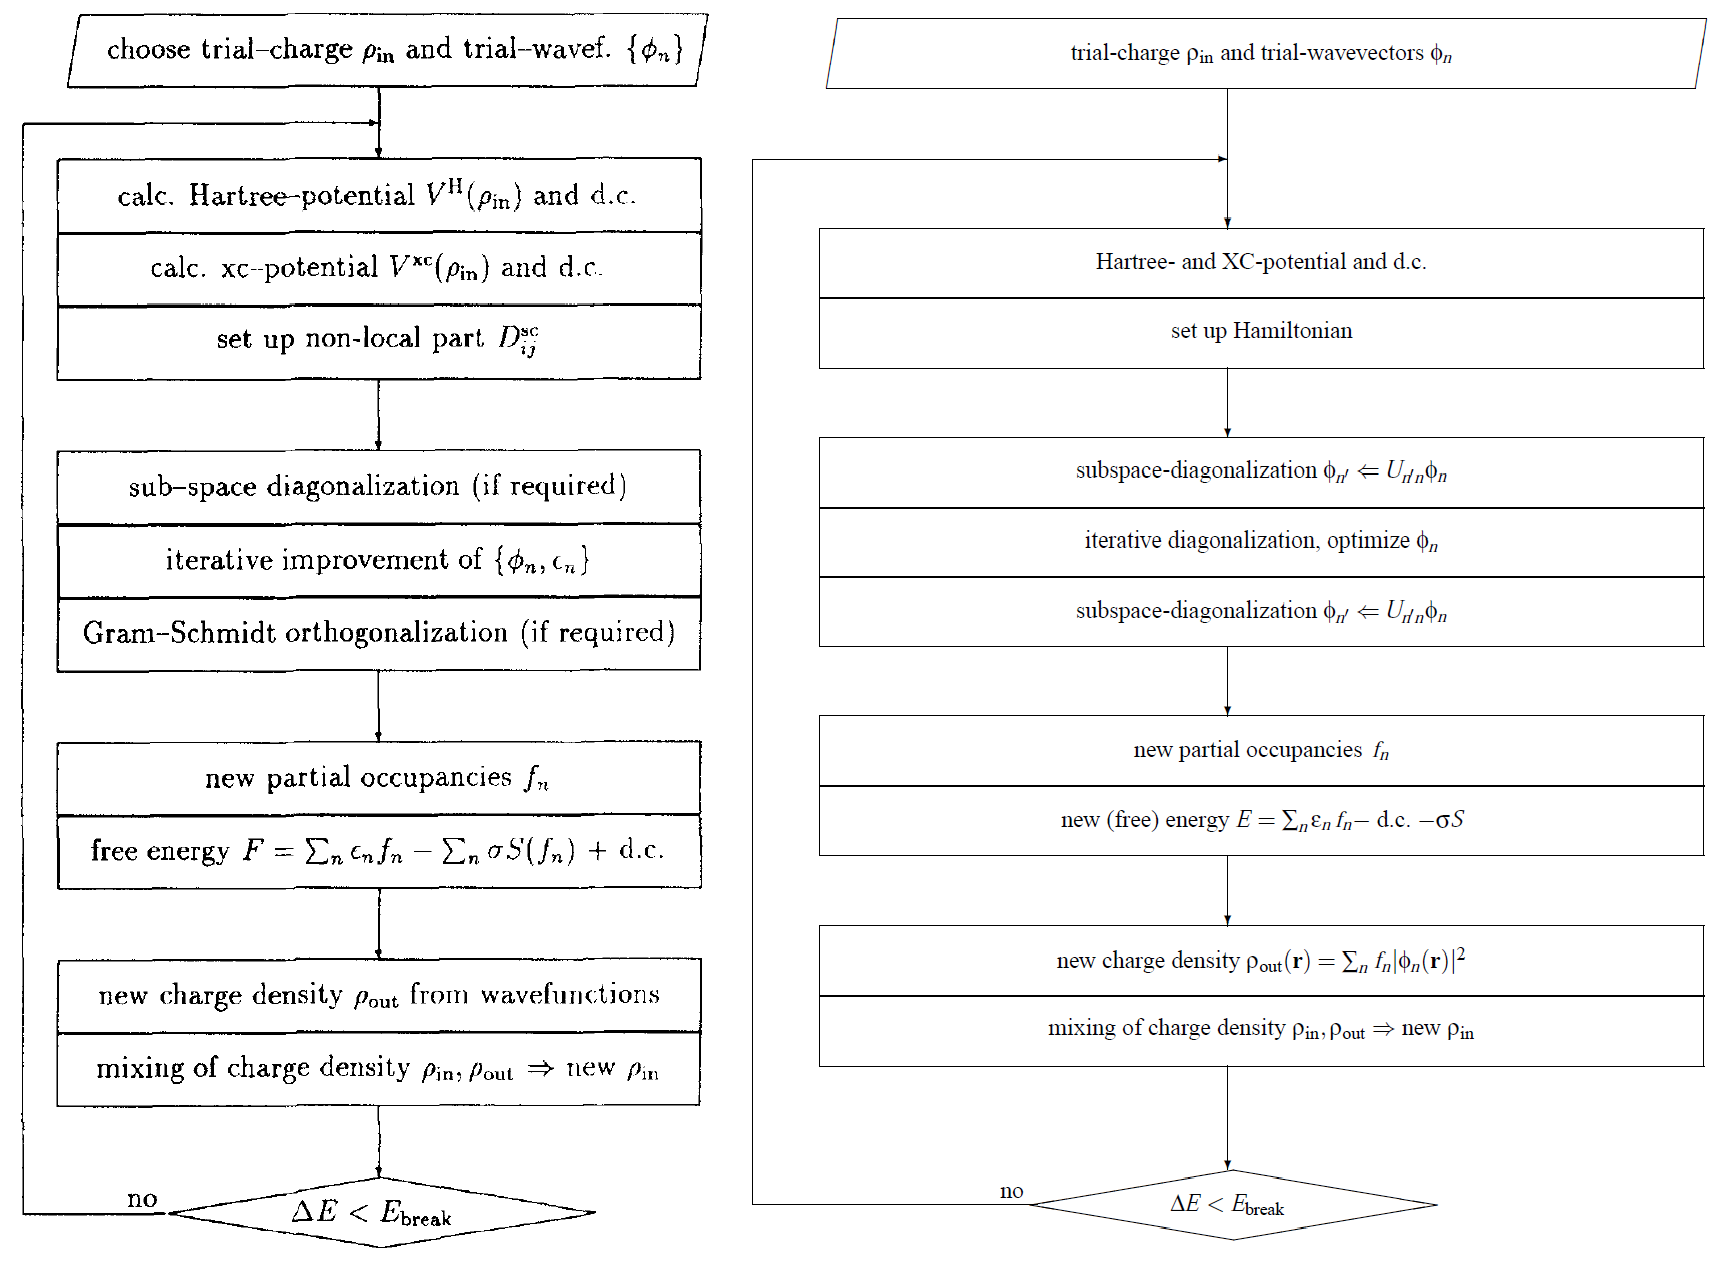
\includegraphics[height=2.7in,width=4.0in,viewport=0 0 1300 960,clip]{Figures/VASP_procedure-full.png}
%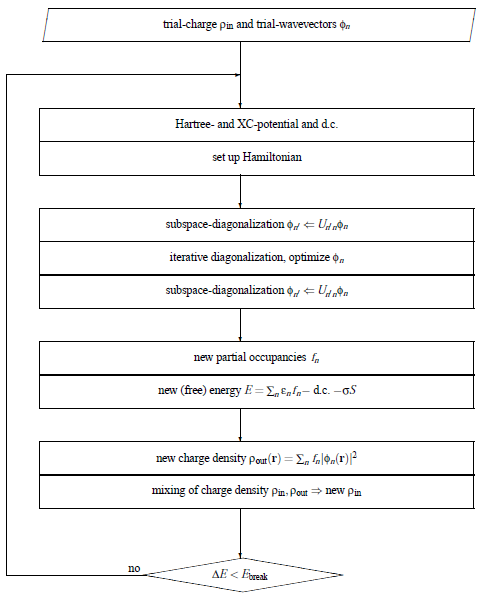
\includegraphics[height=2.1in,width=1.6in,viewport=0 0 480 630,clip]{Figures/VASP_procedure.png}
%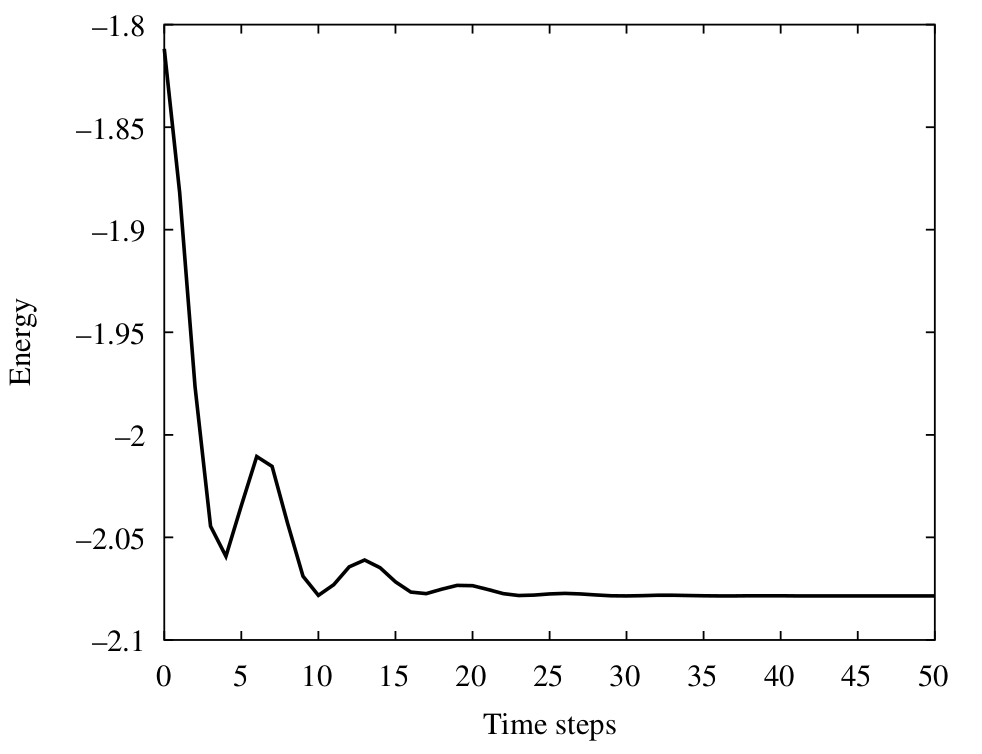
\includegraphics[height=2.1in,width=2.3in,viewport=0 0 740 600,clip]{Figures/Ab-initio-Ene.png}
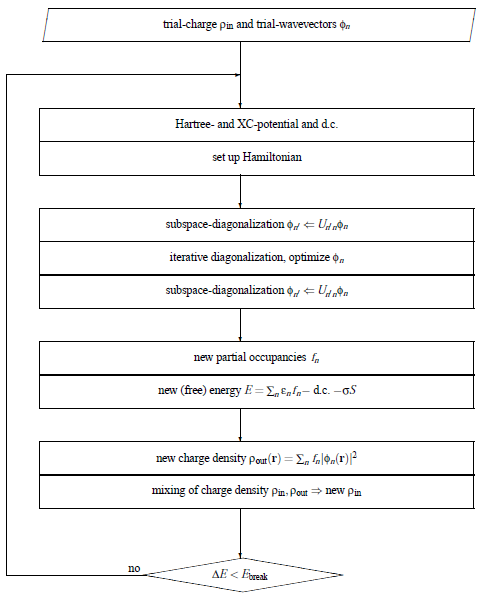
\includegraphics[height=2.5in,width=1.8in,viewport=0 0 480 630,clip]{Figures/VASP_procedure.png}
\caption{\tiny \textrm{The Flow of calculation for the KS-ground states.}}%(与文献\cite{EPJB33-47_2003}图1对比)
\label{PAW_baiseset}
\end{figure} 
}
